\begin{figure*}[t]
  \centering
  \definecolor{fblue}{RGB}{0,114,178}
  \definecolor{forange}{RGB}{230,159,0}
  \definecolor{fverm}{RGB}{213,94,0}
  \definecolor{fink}{RGB}{36,48,57}
  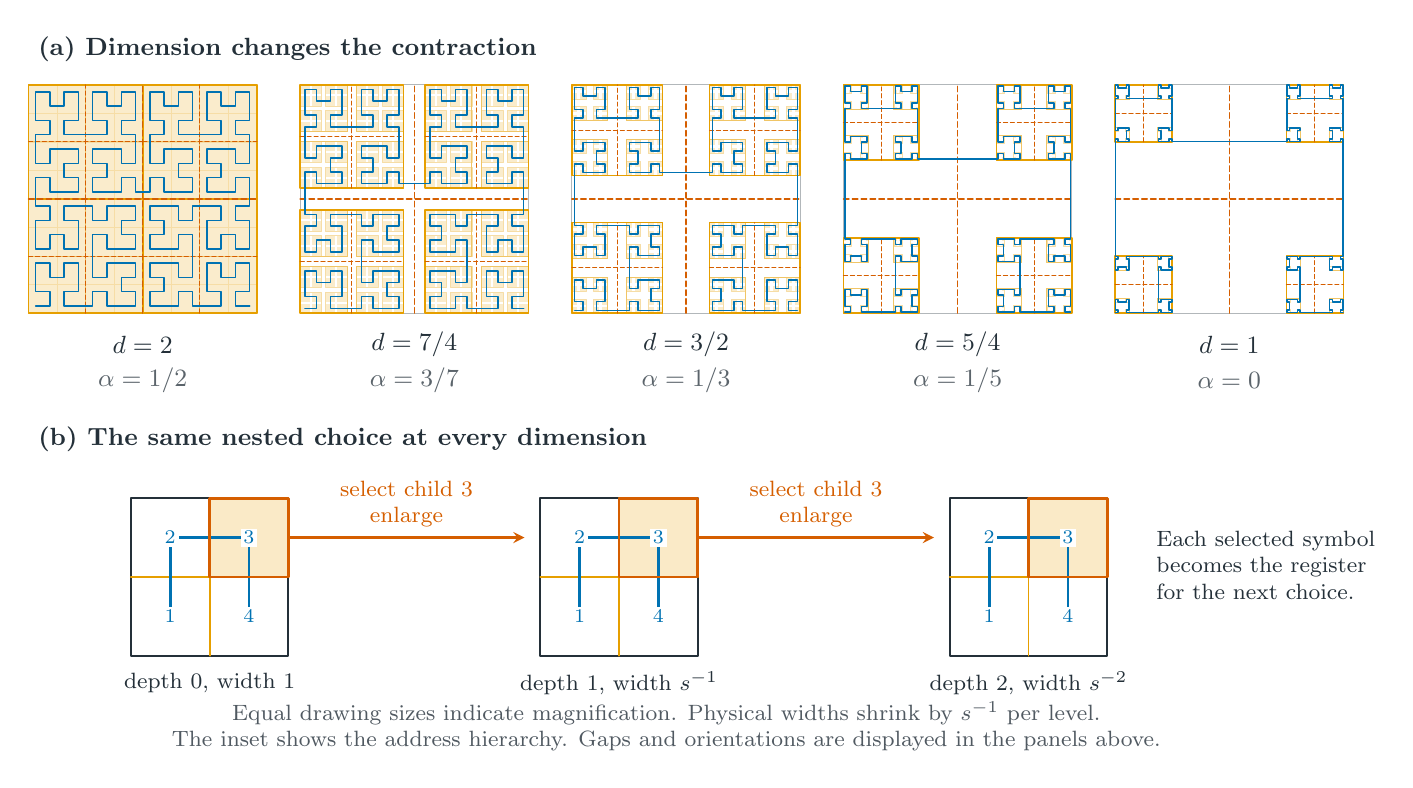
\begin{tikzpicture}[x=1cm,y=1cm,font=\small,line cap=round,line join=round]
  \node[anchor=west,font=\bfseries\small,text=fink] at (0,3.35) {(a) Dimension changes the contraction};
  \def\hsq{2.9}
  \def\cpos#1{(\hsq*((1-1/\hs)*(floor((#1)/8)+mod(floor((#1)/4),2)/\hs+mod(floor((#1)/2),2)/(\hs*\hs)+mod((#1),2)/(\hs*\hs*\hs))))}
  \def\cmid#1{(\cpos{#1}+\hsq/(2*\hs*\hs*\hs*\hs))}
  \def\hlist{0/0,0/1,1/1,1/0,2/0,3/0,3/1,2/1,2/2,3/2,3/3,2/3,1/3,1/2,0/2,0/3,0/4,1/4,1/5,0/5,0/6,0/7,1/7,1/6,2/6,2/7,3/7,3/6,3/5,2/5,2/4,3/4,4/4,5/4,5/5,4/5,4/6,4/7,5/7,5/6,6/6,6/7,7/7,7/6,7/5,6/5,6/4,7/4,7/3,7/2,6/2,6/3,5/3,4/3,4/2,5/2,5/1,4/1,4/0,5/0,6/0,6/1,7/1,7/0}
  \foreach \Dval/\Dlab/\alab [count=\p from 0] in {2/{2}/{1/2},1.75/{7/4}/{3/7},1.5/{3/2}/{1/3},1.25/{5/4}/{1/5},1/{1}/{0}} {
   \pgfmathsetmacro\hs{pow(4,1/\Dval)}
   \begin{scope}[shift={(\p*3.45,0)}]
    \draw[fink!35,line width=0.4pt] (0,0) rectangle (\hsq,\hsq);
    \foreach \i in {0,...,15} \foreach \j in {0,...,15} {
      \pgfmathsetmacro\xc{\cpos{\i}}
      \pgfmathsetmacro\yc{\cpos{\j}}
      \fill[forange!20] (\xc,\yc) rectangle ++({\hsq/(\hs*\hs*\hs*\hs)},{\hsq/(\hs*\hs*\hs*\hs)});
    }
    \foreach \i in {0,...,7} \foreach \j in {0,...,7} {
      \pgfmathsetmacro\xb{\hsq*(1-1/\hs)*(floor(\i/4)+mod(floor(\i/2),2)/\hs+mod(\i,2)/(\hs*\hs))}
      \pgfmathsetmacro\yb{\hsq*(1-1/\hs)*(floor(\j/4)+mod(floor(\j/2),2)/\hs+mod(\j,2)/(\hs*\hs))}
      \draw[forange!35,line width=0.25pt] (\xb,\yb) rectangle ++({\hsq/(\hs*\hs*\hs)},{\hsq/(\hs*\hs*\hs)});
    }
    \foreach \i in {0,...,3} \foreach \j in {0,...,3} {
      \pgfmathsetmacro\xb{\hsq*(1-1/\hs)*(floor(\i/2)+mod(\i,2)/\hs)}
      \pgfmathsetmacro\yb{\hsq*(1-1/\hs)*(floor(\j/2)+mod(\j,2)/\hs)}
      \draw[forange!60,line width=0.35pt] (\xb,\yb) rectangle ++({\hsq/(\hs*\hs)},{\hsq/(\hs*\hs)});
    }
    \foreach \i in {0,1} \foreach \j in {0,1} {
      \pgfmathsetmacro\xa{\hsq*(1-1/\hs)*\i}
      \pgfmathsetmacro\ya{\hsq*(1-1/\hs)*\j}
      \draw[forange,line width=0.6pt] (\xa,\ya) rectangle ++({\hsq/\hs},{\hsq/\hs});
    }
    \draw[fverm,line width=0.5pt,dash pattern=on 2pt off 1.2pt] (\hsq/2,0) -- (\hsq/2,\hsq) (0,\hsq/2) -- (\hsq,\hsq/2);
    \foreach \i in {0,1} \foreach \j in {0,1} {
      \pgfmathsetmacro\xa{\hsq*(1-1/\hs)*\i}
      \pgfmathsetmacro\ya{\hsq*(1-1/\hs)*\j}
      \draw[fverm,line width=0.35pt,dash pattern=on 1.5pt off 1pt] ({\xa+\hsq/(2*\hs)},\ya) -- ++(0,{\hsq/\hs}) (\xa,{\ya+\hsq/(2*\hs)}) -- ++({\hsq/\hs},0);
    }
    \draw[fblue,line width=0.55pt] ({\cmid{0}},{\cmid{0}})
      \foreach \i/\j in \hlist { -- ({\cmid{\j}},{\cmid{\i}}) }
      \foreach \i/\j in \hlist { -- ({\cmid{\i}},{\cmid{\j+8}}) }
      \foreach \i/\j in \hlist { -- ({\cmid{\i+8}},{\cmid{\j+8}}) }
      \foreach \i/\j in \hlist { -- ({\cmid{15-\j}},{\cmid{7-\i}}) };
    \node[text=fink] at (\hsq/2,-0.4) {$d=\Dlab$};
    \node[text=fink!75] at (\hsq/2,-0.85) {$\alpha=\alab$};
   \end{scope}
  }
  % Enlarged address chain: the selected child is a register at the next level.
  \node[anchor=west,text=fink,font=\bfseries\small] at (0,-1.6)
    {(b) The same nested choice at every dimension};
  \foreach \xx/\lev/\widthlab in {1.3/0/{1},6.5/1/{s^{-1}},11.7/2/{s^{-2}}} {
    \begin{scope}[shift={(\xx,-4.35)}]
      \fill[forange!22] (1,1) rectangle (2,2);
      \draw[fink,line width=0.7pt] (0,0) rectangle (2,2);
      \draw[forange,line width=0.7pt] (1,0)--(1,2) (0,1)--(2,1);
      \draw[fblue,line width=1pt] (0.5,0.5)--(0.5,1.5)--(1.5,1.5)--(1.5,0.5);
      \foreach \xxp/\yyp/\lab in {0.5/0.5/1,0.5/1.5/2,1.5/1.5/3,1.5/0.5/4}
        \node[fill=white,inner sep=1pt,text=fblue,font=\scriptsize] at (\xxp,\yyp) {\lab};
      \draw[fverm,line width=1pt] (1,1) rectangle (2,2);
      \node[text=fink,font=\footnotesize] at (1,-0.35) {depth $\lev$, width $\widthlab$};
    \end{scope}
  }
  \draw[->,fverm,line width=0.8pt,>={stealth}]
    (3.3,-2.85) -- (6.3,-2.85)
    node[midway,above,font=\footnotesize,align=center] {select child $3$\\enlarge};
  \draw[->,fverm,line width=0.8pt,>={stealth}]
    (8.5,-2.85) -- (11.5,-2.85)
    node[midway,above,font=\footnotesize,align=center] {select child $3$\\enlarge};
  \node[anchor=west,text=fink,font=\footnotesize,align=left] at (14.2,-3.2)
    {Each selected symbol\\becomes the register\\for the next choice.};
  \node[text=fink!80,font=\footnotesize,align=center] at (8.1,-5.25)
    {Equal drawing sizes indicate magnification. Physical widths shrink by $s^{-1}$ per level.\\
     The inset shows the address hierarchy. Gaps and orientations are displayed in the panels above.};
  \end{tikzpicture}
  \caption{\textbf{The Hilbert order at non-integer dimension.} The
    order-four Hilbert sequence of $N=4^4$ ranks placed on the
    self-similar set generated by four corner maps of ratio $1/s$, with
    $s=4^{1/d}$. Orange outlines mark the registers at depths one to
    three, and shaded cells the individual symbols. Dashed lines are the
    cuts that divide the whole set, and each depth-one register, into
    four. Their lengths are proportional to the width of the register
    divided. The ranks and the nesting are the same in every panel, but
    the registers narrow faster as $d$ falls. With each division priced
    by the length of its cut, $\gamma=1$, the exponent $\alpha=1-1/d$ of
    Eq.~\eqref{eq:geometric-exponent} falls from $1/2$ on Hilbert's
    square to zero, homogeneous refinement, at $d=1$. For $d<2$ the set
    is totally disconnected and the blue path is a guide joining
    consecutive ranks rather than part of the set. The enlarged inset
    follows one address through three levels: the selected child
    (red frame) becomes the register for the next four-way choice.
    This is the same recursion at every $d$, although its physical
    contraction factor $s^{-1}$ differs. Equal inset sizes are
    magnifications, not equal physical register widths.}
  \label{fig:fractional-hilbert}
\end{figure*}
